\section{جهت ۳: نمایش احتمالاتی درجه‌ها}
\label{sec:d3}
\begin{keybox}[شاخه: \branch{direction3-probabilistic-ordinal}]
هر درجه یک \lr{von Mises--Fisher distribution} روی \lr{unit sphere} است: یک \lr{mean direction} که درجه را مکان‌یابی می‌کند و یک \lr{concentration} \lr{trainable} که ابهام آن درجه را نشان می‌دهد. \lr{mixture posterior} این توزیع‌ها جای \lr{softmax} \lr{similarity} را می‌گیرد و هدف دوم، \lr{calibration} احتمال‌هاست.
\end{keybox}

شکل~\ref{fig:wf-d3} گردش کار کامل جهت ۳ را نشان می‌دهد: هر درجه یک \lr{von Mises--Fisher distribution} با \lr{mean direction} و \lr{concentration} \lr{trainable} است و \lr{mixture posterior} آن‌ها جای \lr{softmax} \lr{similarity} را می‌گیرد. \lr{protocol} آزمایش‌ها در شکل~\ref{fig:proto-d3} آمده است.

\begin{landscape}
\begin{figure}[p]
\centering
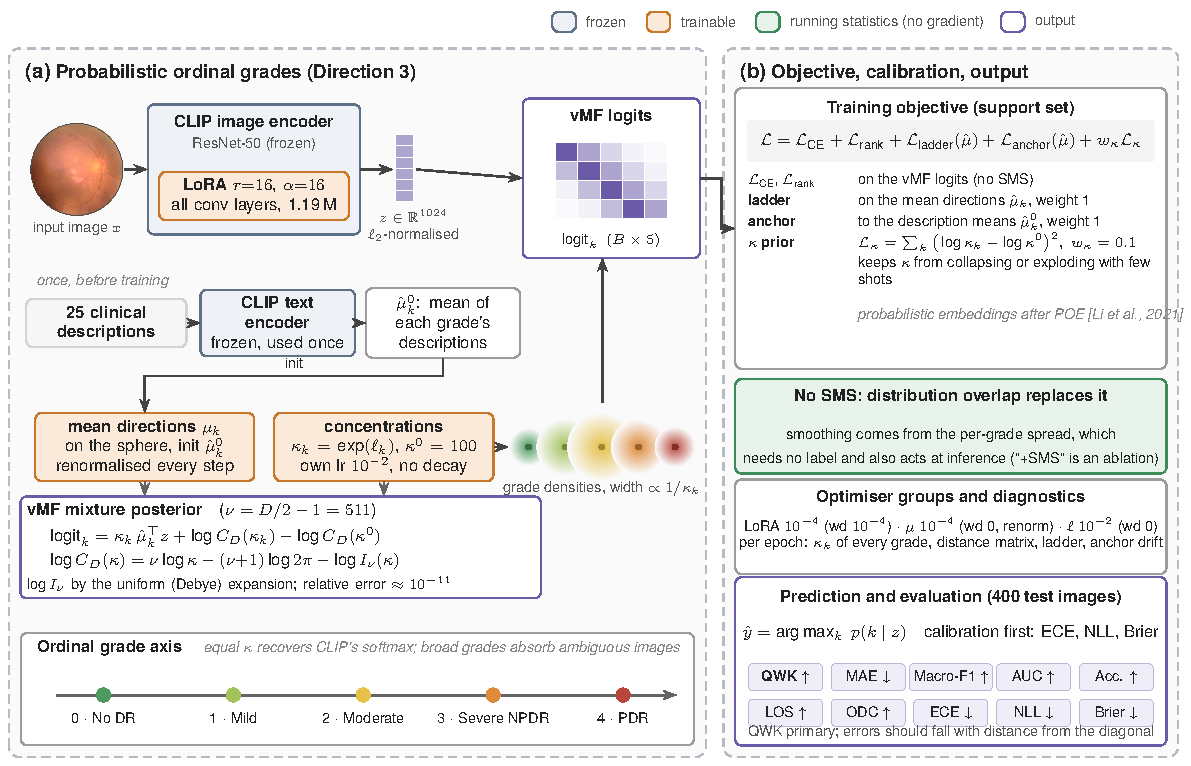
\includegraphics[width=\linewidth]{workflow_d3}
\caption{گردش کار کامل جهت ۳: \lr{mean direction}ها و \lr{concentration}های \lr{trainable}، \lr{mixture posterior} \lr{vMF} با محاسبهٔ پایدار \lr{Bessel function}، \lr{loss function} با \lr{concentration prior} و تأکید بر \lr{metric}های \lr{calibration}.}
\label{fig:wf-d3}
\end{figure}
\end{landscape}

% ------------------------------------------------------------------
\subsection{انگیزه و شکاف پژوهشی}
مرز درجه‌های \lr{DR} قطعی نیست و اختلاف نظر درجه‌بندها بیشتر میان درجه‌های ۱ و ۲ و میان ۲ و ۳ دیده می‌شود. یک \lr{prototype} تک‌نقطه‌ای نمی‌تواند این ابهام را نشان دهد. در جهت ۳ هر درجه یک توزیع روی \lr{unit sphere} است: یک \lr{mean direction} که درجه را مکان‌یابی می‌کند و یک \lr{concentration} که نشان می‌دهد درجه چقدر روشن تعریف شده است. نمایش احتمالاتی پیش‌تر در سمت تصویر بررسی شده است (\lr{POE} \cite{poe})، اما \lr{prototype}ها احتمالاتی سمت متن با \lr{constraint} ترتیبی، برای درجه‌بندی \lr{few-shot}، در مرور منابع این پژوهش یافت نشد. هدف دوم این جهت \lr{calibration} است: احتمال‌هایی که با دقت واقعی هم‌خوانی دارند، برای کاربرد بالینی ارزشمندند.

\begin{figure}[H]
\centering
\begin{latin}
\begin{tikzpicture}[x=-1cm,y=1cm]
  \begin{scope}
    \foreach \x/\n in {0/0,-1.6/1,-3.2/2,-4.8/3,-6.4/4} {\fill[accent] (\x,0) circle (3pt); \node[below=3pt,font=\footnotesize] at (\x,0) {\n};}
    \node[font=\footnotesize\bfseries] at (-3.2,0.9) {Point prototype};
  \end{scope}
  \begin{scope}[yshift=-2.6cm]
    \foreach \x/\w/\n in {0/0.45/0,-1.6/0.75/1,-3.2/0.95/2,-4.8/0.7/3,-6.4/0.5/4} {
      \shade[inner color=accent!70,outer color=white] (\x,0) circle (\w);
      \fill[accent] (\x,0) circle (2pt); \node[below=\w cm,font=\footnotesize] at (\x,0) {\n};}
    \node[font=\footnotesize\bfseries] at (-3.2,1.3) {Distribution with per-grade concentration};
  \end{scope}
\end{tikzpicture}
\end{latin}
\caption{از نقطه به توزیع: درجه‌های مبهم‌تر (مانند ۱ تا ۳) می‌توانند \lr{concentration} کمتر و پراکندگی بیشتری بیاموزند.}
\label{fig:d3-idea}
\end{figure}

% ------------------------------------------------------------------
\subsection{مدل \lr{von Mises--Fisher} برای هر درجه}
\lr{von Mises--Fisher distribution} (\lr{vMF}) روی \lr{sphere} $S^{D-1}$ با \lr{mean direction} $\mu$ و \lr{concentration} $\kappa$ چنین است:
\begin{equation}
\mathrm{vMF}(z;\, \mu, \kappa) = C_D(\kappa)\, \exp(\kappa\, \mu^{\top} z), \qquad C_D(\kappa) = \frac{\kappa^{\nu}}{(2\pi)^{\nu+1} I_{\nu}(\kappa)}, \qquad \nu = \frac{D}{2} - 1 = 511
\label{eq:vmf}
\end{equation}
تابع $I_\nu$ \lr{modified Bessel function of the first kind} است. برای هر درجه، $\mu_k$ مانند جهت ۱ یک بردار آزاد روی \lr{sphere} است که از میانگین ۲۵ توصیف بالینی جهت ۲ (با \lr{encoder} \lr{frozen}) آغاز می‌شود، و $\kappa_k = \exp(\ell_k)$ با مقدار اولیهٔ ۱۰۰ آموخته می‌شود. این مقدار اولیه همان \lr{logit scale} \lr{CLIP} است.

% ------------------------------------------------------------------
\subsection{امتیازدهی: \lr{mixture posterior} \lr{vMF}}
تصویر با \lr{mixture posterior}‌ای از پنج توزیع طبقه‌بندی می‌شود. ثابت $\log C_D(\kappa^{0})$ برای همهٔ درجه‌ها یکسان است و در \lr{softmax} حذف می‌شود؛ کم کردن آن در \lr{double precision}، \lr{logit}ها را در مقیاس \lr{CLIP} نگه می‌دارد. مقدار $\log C_D$ در $\kappa=100$ حدود ۲۰۰۰+ است و جمع آن در \lr{single precision} حدود چهار رقم اعشار را از بین می‌برد:
\begin{equation}
\mathrm{logit}_k = \kappa_k\, \hat{\mu}_k^{\top} z + \log C_D(\kappa_k) - \log C_D(\kappa^{0}), \qquad p(k \mid z) = \operatorname{softmax}_k(\mathrm{logit}_k)
\label{eq:vmf-logit}
\end{equation}
دو ویژگی این امتیازدهی مهم است:
\begin{enumerate}[label=\arabic*.]
\item اگر همهٔ $\kappa_k$ برابر باشند، \lr{posterior} دقیقاً \lr{softmax} \lr{similarity} \lr{CLIP} با مقیاس $\kappa$ است؛ پس حالت \lr{zero-shot} همان \lr{classifier} \lr{zero-shot} با میانگین توصیف‌هاست.
\item اگر درجه‌ای پهن‌تر شود ($\kappa$ کمتر)، برای تصاویری که از همهٔ میانگین‌ها دورند احتمال بیشتری می‌گیرد؛ این همان رفتار هموارسازی است که \lr{SMS} به \lr{similarity}ها تحمیل می‌کند، اما اینجا جزء خود مدل است و در آزمون هم وجود دارد.
\end{enumerate}
در \lr{ablation}، امتیازدهی دیگری هم بررسی می‌شود: \lr{similarity} مورد انتظار با \lr{prototype}‌ای که از توزیع درجه برداشته شود. نسبت $A_D(\kappa) = I_{\nu+1}(\kappa) / I_{\nu}(\kappa)$ \lr{mean resultant length} است؛ برای نمونه $A_D(100) \approx 0.0967$ که با مقیاس \lr{similarity}های واقعی \lr{CLIP} هم‌خوانی دارد:
\begin{equation}
\mathrm{logit}_k = 100 \cdot \frac{A_D(\kappa_k)}{A_D(\kappa^{0})}\, \hat{\mu}_k^{\top} z
\label{eq:expected}
\end{equation}

% ------------------------------------------------------------------
\subsection{محاسبهٔ پایدار \lr{Bessel function}}
در مرتبهٔ $\nu=511$ تابع $I_\nu$ در دقت معمولی فرومی‌ریزد؛ برای نمونه، تابع \code{scipy.special.iv} در $\kappa=50$ مقدار صفر و در $\kappa=100$ مقداری از مرتبهٔ $10^{-294}$ برمی‌گرداند. به همین دلیل لگاریتم آن با \lr{uniform asymptotic expansion} (\lr{Debye expansion}) و نخستین جملهٔ تصحیحی محاسبه می‌شود \cite{dlmf}:
\begin{equation}
\begin{aligned}
\log I_{\nu}(\kappa) &\approx \eta - \tfrac{1}{2}\log(2\pi) - \tfrac{1}{4}\log(\nu^2 + \kappa^2) + \log\!\Big(1 + \frac{u_1(t)}{\nu}\Big),\\
\eta &= \sqrt{\nu^2 + \kappa^2} + \nu \log \frac{\kappa}{\nu + \sqrt{\nu^2 + \kappa^2}}, \qquad t = \frac{\nu}{\sqrt{\nu^2 + \kappa^2}}, \qquad u_1(t) = \frac{3t - 5t^3}{24}
\end{aligned}
\label{eq:bessel}
\end{equation}
این تقریب در بازهٔ $\kappa \in [1, 1000]$ با محاسبهٔ دقت دلخواه کتابخانهٔ \lr{mpmath} مقایسه شده و \lr{relative error} آن حدود $10^{-11}$ است. تقریب نسبت به $\kappa$ هموار و مشتق‌پذیر است و \lr{gradient} مستقیماً از آن عبور می‌کند.

\begin{figure}[H]
\begin{diagram}
  \node[train=2.4cm] (k) {$\ell_k$};
  \node[box=2.4cm,right=of k] (e) {$\kappa_k=e^{\ell_k}$};
  \node[box=3.6cm,right=of e] (b) {$\log I_\nu(\kappa_k)$\\ Debye expansion, Eq.~\ref{eq:bessel}};
  \node[box=3cm,below=of b] (c) {$\log C_D(\kappa_k)$\\ Eq.~\ref{eq:vmf}};
  \node[box=3cm,left=of c] (c0) {Subtract $\log C_D(\kappa^0)$ in float64};
  \node[lossn=3.2cm,left=of c0] (lg) {Logit, Eq.~\ref{eq:vmf-logit}};
  \draw[arr] (k)--(e); \draw[arr] (e)--(b); \draw[arr] (b)--(c); \draw[arr] (c)--(c0); \draw[arr] (c0)--(lg);
\end{diagram}
\caption{مسیر محاسبهٔ \lr{logit} \lr{vMF}. \lr{gradient} از همهٔ مراحل تا $\ell_k$ عبور می‌کند.}
\label{fig:d3-bessel}
\end{figure}

% ------------------------------------------------------------------
\subsection{معماری}
\begin{figure}[H]
\begin{diagram}
  \node[datan=3cm] (d) {25 clinical descriptions};
  \node[frozen=3cm,right=7mm of d] (te) {Frozen text encoder};
  \node[datan=3cm,right=7mm of te] (m0) {$\mu^0_k$: mean of descriptions per grade};
  \node[train=3.4cm,below=12mm of m0] (mu) {$\mu_k$: mean direction, free on sphere};
  \node[train=3.4cm,left=6mm of mu] (ka) {$\kappa_k=\exp(\ell_k)$: concentration per grade\\ init: $\kappa^0=100$};
  \node[datan=2.4cm,left=12mm of ka] (x) {Image};
  \node[train=2.8cm,below=of x] (v) {CLIP RN50 + LoRA};
  \node[box=4cm,below=14mm of ka] (p) {vMF mixture posterior\\ Eq.~\ref{eq:vmf-logit}};
  \node[lossn=3cm,below=of p] (l1) {CE + rank-aware loss};
  \node[lossn=3cm,right=5mm of l1] (l2) {Ladder + anchor on $\mu$};
  \node[lossn=3cm,left=5mm of l1] (l3) {Log-normal prior on $\kappa$};
  \node[datan=5cm,below=of l1] (o) {Calibrated probs: ECE · NLL · Brier};
  \draw[arr] (d)--(te); \draw[arr] (te)--(m0); \draw[arr] (m0)--node[elabel,right]{init}(mu);
  \draw[arr] (x)--(v); \draw[arr] (v) |- node[elabel,above,pos=0.75]{$z$} (p.west);
  \draw[arr] (mu) |- (p.east); \draw[arr] (ka)--(p);
  \draw[arr] (p)--(l1); \draw[arr] (mu.south) -- (mu.south |- l2.north); \draw[arr] (ka.west) -- ++(-4mm,0) |- (l3.north);
  \draw[arr] (l1)--(o);
  \begin{scope}[on background layer]\node[group,fit=(d)(te)(m0)] (gi) {};\end{scope}
  \node[grouplabel,anchor=south] at (gi.north) {Once, before training};
\end{diagram}
\archlegend
\caption{معماری جهت ۳. هر درجه دو جزء \lr{trainable} دارد: \lr{mean direction} و \lr{concentration}.}
\label{fig:d3-arch}
\end{figure}

% ------------------------------------------------------------------
\subsection{\lr{loss function}ها}
\lr{loss} \lr{CE} و \lr{ranking-aware loss} روی \lr{logit}های \lr{vMF} محاسبه می‌شوند. \lr{constraint}های \lr{ladder} (رابطهٔ~\ref{eq:ladder}) و \lr{anchor} (رابطهٔ~\ref{eq:anchor}) روی \lr{mean direction}ها اعمال می‌شوند. برای \lr{concentration}ها یک \lr{prior} \lr{log}-نرمال وجود دارد، چون در \lr{regime} \lr{few-shot} $\kappa$ بدون \lr{constraint} می‌تواند فرو بریزد یا منفجر شود:
\begin{equation}
\mathcal{L} = \mathcal{L}_{\mathrm{CE}} + \mathcal{L}_{\mathrm{rank}} + \mathcal{L}_{\mathrm{ladder}}(\hat{\mu}) + \mathcal{L}_{\mathrm{anchor}}(\hat{\mu}) + w_{\kappa} \sum_k \big(\log \kappa_k - \log \kappa^{0}\big)^2, \qquad w_{\kappa} = 0.1
\label{eq:d3-loss}
\end{equation}
\lr{SMS} در مدل اصلی خاموش است، چون نقش آن را \lr{overlap} توزیع‌ها بر عهده دارد؛ نسخهٔ «+ \lr{SMS}» در \lr{ablation} این فرض را می‌آزماید. \lr{constraint} \lr{path} و \lr{pairwise loss} هم خاموش‌اند.

\begin{table}[H]
\caption{اجزای \lr{loss function} جهت ۳}
\label{tab:d3-loss}
\centering\small
\begin{tabularx}{\textwidth}{@{}p{3.2cm} p{2.6cm} c X@{}}
\toprule
\textbf{جزء} & \textbf{روی چه چیزی} & \textbf{وزن} & \textbf{نقش}\\
\midrule
\lr{cross-entropy} & \lr{logit} \lr{vMF} & ۱ & طبقه‌بندی درست\\
\lr{ranking-aware loss} & \lr{logit} \lr{vMF} & ۱ & شکل \lr{unimodal} \lr{posterior}\\
\lr{ladder} & $\hat\mu_k$ & ۱ & ترتیب فاصلهٔ \lr{mean direction}ها\\
\lr{anchor} & $\hat\mu_k,\hat\mu^0_k$ & ۱ & حفظ دانش زبانی\\
\lr{concentration prior} & $\log\kappa_k$ & \LRE{۰٫۱} & جلوگیری از فروریختن یا انفجار $\kappa$\\
\bottomrule
\end{tabularx}
\end{table}

% ------------------------------------------------------------------
\subsection{بهینه‌سازی}
\lr{mean direction}ها با نرخ $10^{-4}$، بدون \lr{weight decay} و با \lr{normalisation} پس از هر گام آموخته می‌شوند. لگاریتم \lr{concentration}ها گروه جداگانه‌ای با نرخ $10^{-2}$ و بدون \lr{weight decay} دارند. دلیل نرخ جداگانه این است که $\log\kappa$ حدود \LRE{۴٫۶} است و با نرخ عمومی $10^{-4}$ در طول ۵۰ \lr{epoch} تقریباً ثابت می‌ماند. \lr{parameter}های \lr{trainable} \LRE{۱٬۱۸۸٬۲۷۲} + \LRE{۵٬۱۲۰} + ۵ = \LRE{۱٬۱۹۳٬۳۹۷} است.

\begin{table}[H]
\caption{گروه‌های \lr{parameter} در \lr{optimizer} جهت ۳}
\label{tab:d3-opt}
\centering\small
\begin{tabular}{@{}lcccc@{}}
\toprule
\textbf{گروه} & \textbf{تعداد} & \textbf{\lr{learning rate}} & \textbf{\lr{weight decay}} & \textbf{پس از هر گام}\\
\midrule
\lr{LoRA} تصویر & \LRE{۱٬۱۸۸٬۲۷۲} & $10^{-4}$ & $10^{-4}$ & --\\
\lr{mean direction}ها $\mu$ & \LRE{۵٬۱۲۰} & $10^{-4}$ & ۰ & \lr{normalisation}\\
لگاریتم \lr{concentration} $\ell$ & ۵ & $10^{-2}$ & ۰ & --\\
\bottomrule
\end{tabular}
\end{table}

% ------------------------------------------------------------------
\subsection{داده، ارزیابی و تأکید بر \lr{calibration}}
داده، \lr{protocol} ۲۴ اجرایی و همهٔ \lr{metric}های بخش~\ref{sec:metrics} بدون تغییر به کار می‌روند. چون ادعای اصلی این جهت \lr{calibration} است، جدول‌ها و منحنی‌های $k$ افزون بر \lr{QWK}، \lr{MAE} و \lr{ODC}، \lr{metric}های \lr{ECE} و \lr{NLL} را هم برای همهٔ مدل‌ها نشان می‌دهند و \lr{Brier score} هم گزارش می‌شود. تشخیص‌های هر \lr{epoch} علاوه بر ماتریس فاصله، \lr{ladder} و فاصله از \lr{anchor}، مقدار $\kappa$ هر درجه را هم ثبت می‌کند؛ مسیر تغییر $\kappa$ نشان می‌دهد مدل کدام درجه‌ها را مبهم‌تر یافته است.

% ------------------------------------------------------------------
\subsection{\lr{baseline}ها و \lr{ablation}ها}
مرجع اصلی مقایسه \lr{CLIP-DR} \lr{matched} است، چون \lr{SMS} همان جزئی است که جهت ۳ جایگزینش می‌کند. مدل \lr{master}، جهت‌های ۱ و ۲، مدل‌های جدول~\ref{tab:baselines} و \lr{CLIP-LoRA} با \lr{loss}های ترتیبی هم در مقایسه حضور دارند.

\begin{table}[H]
\caption{\lr{ablation}ها جهت ۳}
\label{tab:d3-abl}
\centering\small
\begin{tabularx}{\textwidth}{@{}p{3.8cm} X X@{}}
\toprule
\textbf{آزمایش} & \textbf{تغییر} & \textbf{پرسشی که پاسخ می‌دهد}\\
\midrule
$\kappa$ مشترک & یک \lr{concentration} برای همهٔ درجه‌ها (یک دمای \lr{trainable}) & آیا ابهام جداگانهٔ هر درجه لازم است؟\\
$\kappa$ ثابت & \lr{concentration} آموخته نمی‌شود & مدل قطعی با همان مقداردهی\\
\lr{similarity} مورد انتظار & رابطهٔ~\ref{eq:expected} به‌جای \ref{eq:vmf-logit} & کدام امتیازدهی بهتر است؟\\
+ \lr{SMS} & افزودن \lr{SMS} & آیا \lr{overlap} توزیع‌ها جای \lr{SMS} را می‌گیرد؟\\
بدون \lr{ladder} / \lr{anchor} / \lr{prior} $\kappa$ & وزن همان جزء صفر & سهم هر \lr{constraint}\\
مقداردهی با یک جملهٔ بالینی & جملهٔ جهت ۱ به‌جای میانگین ۵ توصیف & اثر میانگین‌گیری توصیف‌ها\\
$\kappa^{0} = 50$ & توزیع‌های پهن‌تر در آغاز & حساسیت به مقدار اولیه\\
+ \lr{pairwise loss} & افزودن \lr{distance-weighted pairwise loss} & سهم این \lr{loss} در جهت ۳\\
\bottomrule
\end{tabularx}
\end{table}

\begin{figure}[H]
\centering
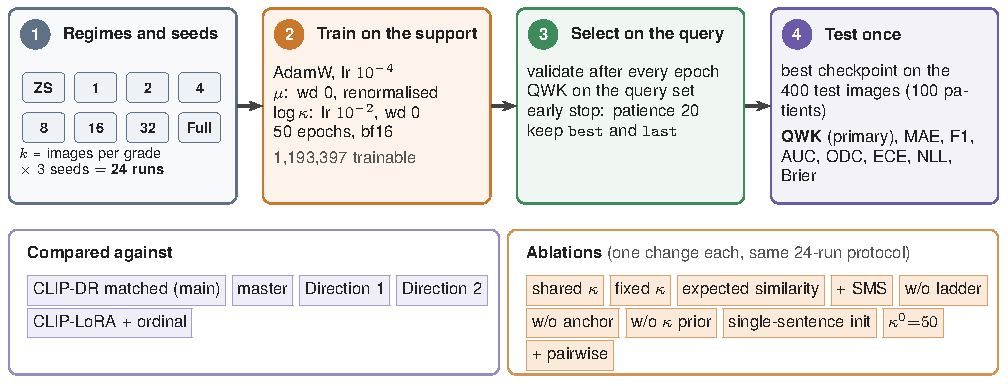
\includegraphics[width=\linewidth]{protocol_d3}
\caption{\lr{protocol} آزمایش‌های جهت ۳.}
\label{fig:proto-d3}
\end{figure}

\begin{figure}[H]
\begin{diagram}
  \node[train=4.4cm] (a) {Phase 1: Dir.~3 · 24 runs};
  \node[box=4.4cm,below=of a] (b) {Compare main models\\ QWK · ODC · ECE · NLL};
  \node[decision,below=of b] (c) {Dir.~3 is best?};
  \node[train=5cm,below=of c] (d) {Phase 2: compare with CLIP-DR \& others + 11 ablations};
  \node[lossn=5cm,below=of d] (e) {Calibration tables and $\kappa$ trajectory per grade};
  \draw[arr] (a)--(b); \draw[arr] (b)--(c); \draw[arr] (c)--node[elabel,right]{yes}(d); \draw[arr] (d)--(e);
\end{diagram}
\caption{گردش کار آزمایش‌های جهت ۳.}
\label{fig:d3-flow}
\end{figure}
